\documentclass{article}
\usepackage[utf8]{inputenc}
\usepackage{comment}
\usepackage{hyperref}
\usepackage{natbib}
\usepackage{listings}
\usepackage{verbatim}
\usepackage{adjustbox}
\bibliographystyle{dinat}
\usepackage{tikz}
\usetikzlibrary{shapes.geometric, arrows}
\usepackage{graphicx}
\graphicspath{ {./images/} }


\title{Scalable Clustering of COVID-19 Mobility Data }
\author{Daniel~Achee\and Can~Aygun \and Bobby~Judd \and Josh~Kimmel \and Zixuan~Zhong}

\date{UCLA | CS 216 | June 2020}

\begin{document}
\maketitle

\section{Introduction}
We have implemented the scalable clustering algorithm described in \cite{sc-paper}.  In the following sections we describe our implementation, chosen dataset, and results.

\section{Software Architecture}
In section 2.1 to 2.6, we describe the main components of the software that implements the scalable clustering algorithm.The GitHub repository for this project can be found at: \\ \url{https://github.com/joshkimmel16/scalable-clustering}

\subsection{Config}

The config module allows users to customize the application of the algorithm to their specific use cases and data sets. In that spirit, the following parameters are supported:
\begin{itemize}
  \item \textbf{DATA\_PATH}: Path to input data set. Data sets are assumed to be of the .csv format. (String)
  \item \textbf{DATA\_START}: The first row of actual data in the input data set file. (Int)
  \item \textbf{NUM\_ATTRS}: The number of columns that are included in the clustering algorithm (equal to the number of dimensions in the graph). (Int)
  \item \textbf{DATA\_INDICES}: The columns (0-indexed) that are relevant for clustering. All other columns are ignored. (Comma-Separated List of Ints)
  \item \textbf{DATA\_TYPES}: The type of each column included in the clustering algorithm. See \nameref{DataTypes} for a list of supported types. (Comma-Separated List of Data Types)
  \item \textbf{NULL\_ACTION}: The action to take when a null value is encountered for a column included in the clustering algorithm. See \nameref{NullActions} for a list of supported actions. (Null action)
  \item \textbf{DEFAULT\_VALS}: The default values for all included columns to be used if a null value is encountered. Only honored if NULL\_ACTION is ACTION\_DEFAULT. (Comma-Separated List of Strings)
  \item \textbf{CUTOFF\_VALS}: The values for each column to use for branching (to create clusters in the cluster graph). (Comma-Separated List of Arrays of Strings)
  \item \textbf{THRESHOLD}: The threshold count that defines "interesting" clusters. (Double)
  \item \textbf{BATCH\_SIZE}: The numbers of row that will be read into memory at any given time. (Int)
  \item \textbf{REPORT\_PATH}: The path to the output report file. (String)
\end{itemize}

\subsubsection{Data Types}
\label{DataTypes}

The following data types are currently supported:
\begin{itemize}
    \item \textbf{DATA\_STRING}: Standard string. Uses traditional string comparisons.
    \item \textbf{DATA\_INT}: Integer. Uses traditional int comparisons.
    \item \textbf{DATA\_DOUBLE}: Double. Uses traditional double comparisons.
    \item \textbf{DATA\_DATE}: Date (assumed to be yyyy-mm-dd).
\end{itemize}

\subsubsection{Null Actions}
\label{NullActions}

The following null actions are currently supported:

\begin{itemize}
    \item \textbf{ACTION\_OMIT}: Omit any row in which any column included in the clustering algorithm has a null value.
    \item \textbf{ACTION\_DEFAULT}: Replace any encountered null value with a provided default value (specified in the DEFAULT\_VALS config parameter)
\end{itemize}

\subsection{Compare}

The compare module defines how data attributes of different types are compared for the purposes of cluster graph traversal. This module is key to the user's ability to extend our application to arbitrary data sets.

To support a new data type, the user must simply extend this module to define a new comparison function. From there, specifying this new data type in the config will allow the algorithm to properly use columns of this type.

\subsection{DataPoint}

DataPoints are the atomic unit of comparison in the algorithm. They can be thought of as k-dimensional vectors where k is the number of columns/attributes used for clustering. Each (non-omitted) row in the data set is parsed into a DataPoint object before traversing the cluster graph.

\subsection{ClusterGraph}

The clustergraph module has two major classes: Cluster and ClusterGraph. A lot of Cluster objects form a multi-dimensional tree and ClusterGraph holds the root of the tree. 

For each dimension, the Cluster object has one parent and two (left and right) children. Hence, if it is a k-dimensional graph, each Cluster object will have k parents and 2k children in general.

The graph is built once the config module has read the parameters from the configuration file successfully. 

\subsubsection{Cutoff Values and Anchors}

If the cutoff values from the configuration file for a dimension is \([a,b,c,d,e,f,g,h,i,j,k]\), we create an augmented array, called cutoffs, by appending an infinity value to the end of the array so that cutoffs = \([a,b,c,d,e,f,g,h,i,j,k,\infty]\) in this case. 

The root and other nodes will divide the array into two even sub-arrays if the length is greater than 1. The tree for this dimension looks like this diagram.

\begin{center}
   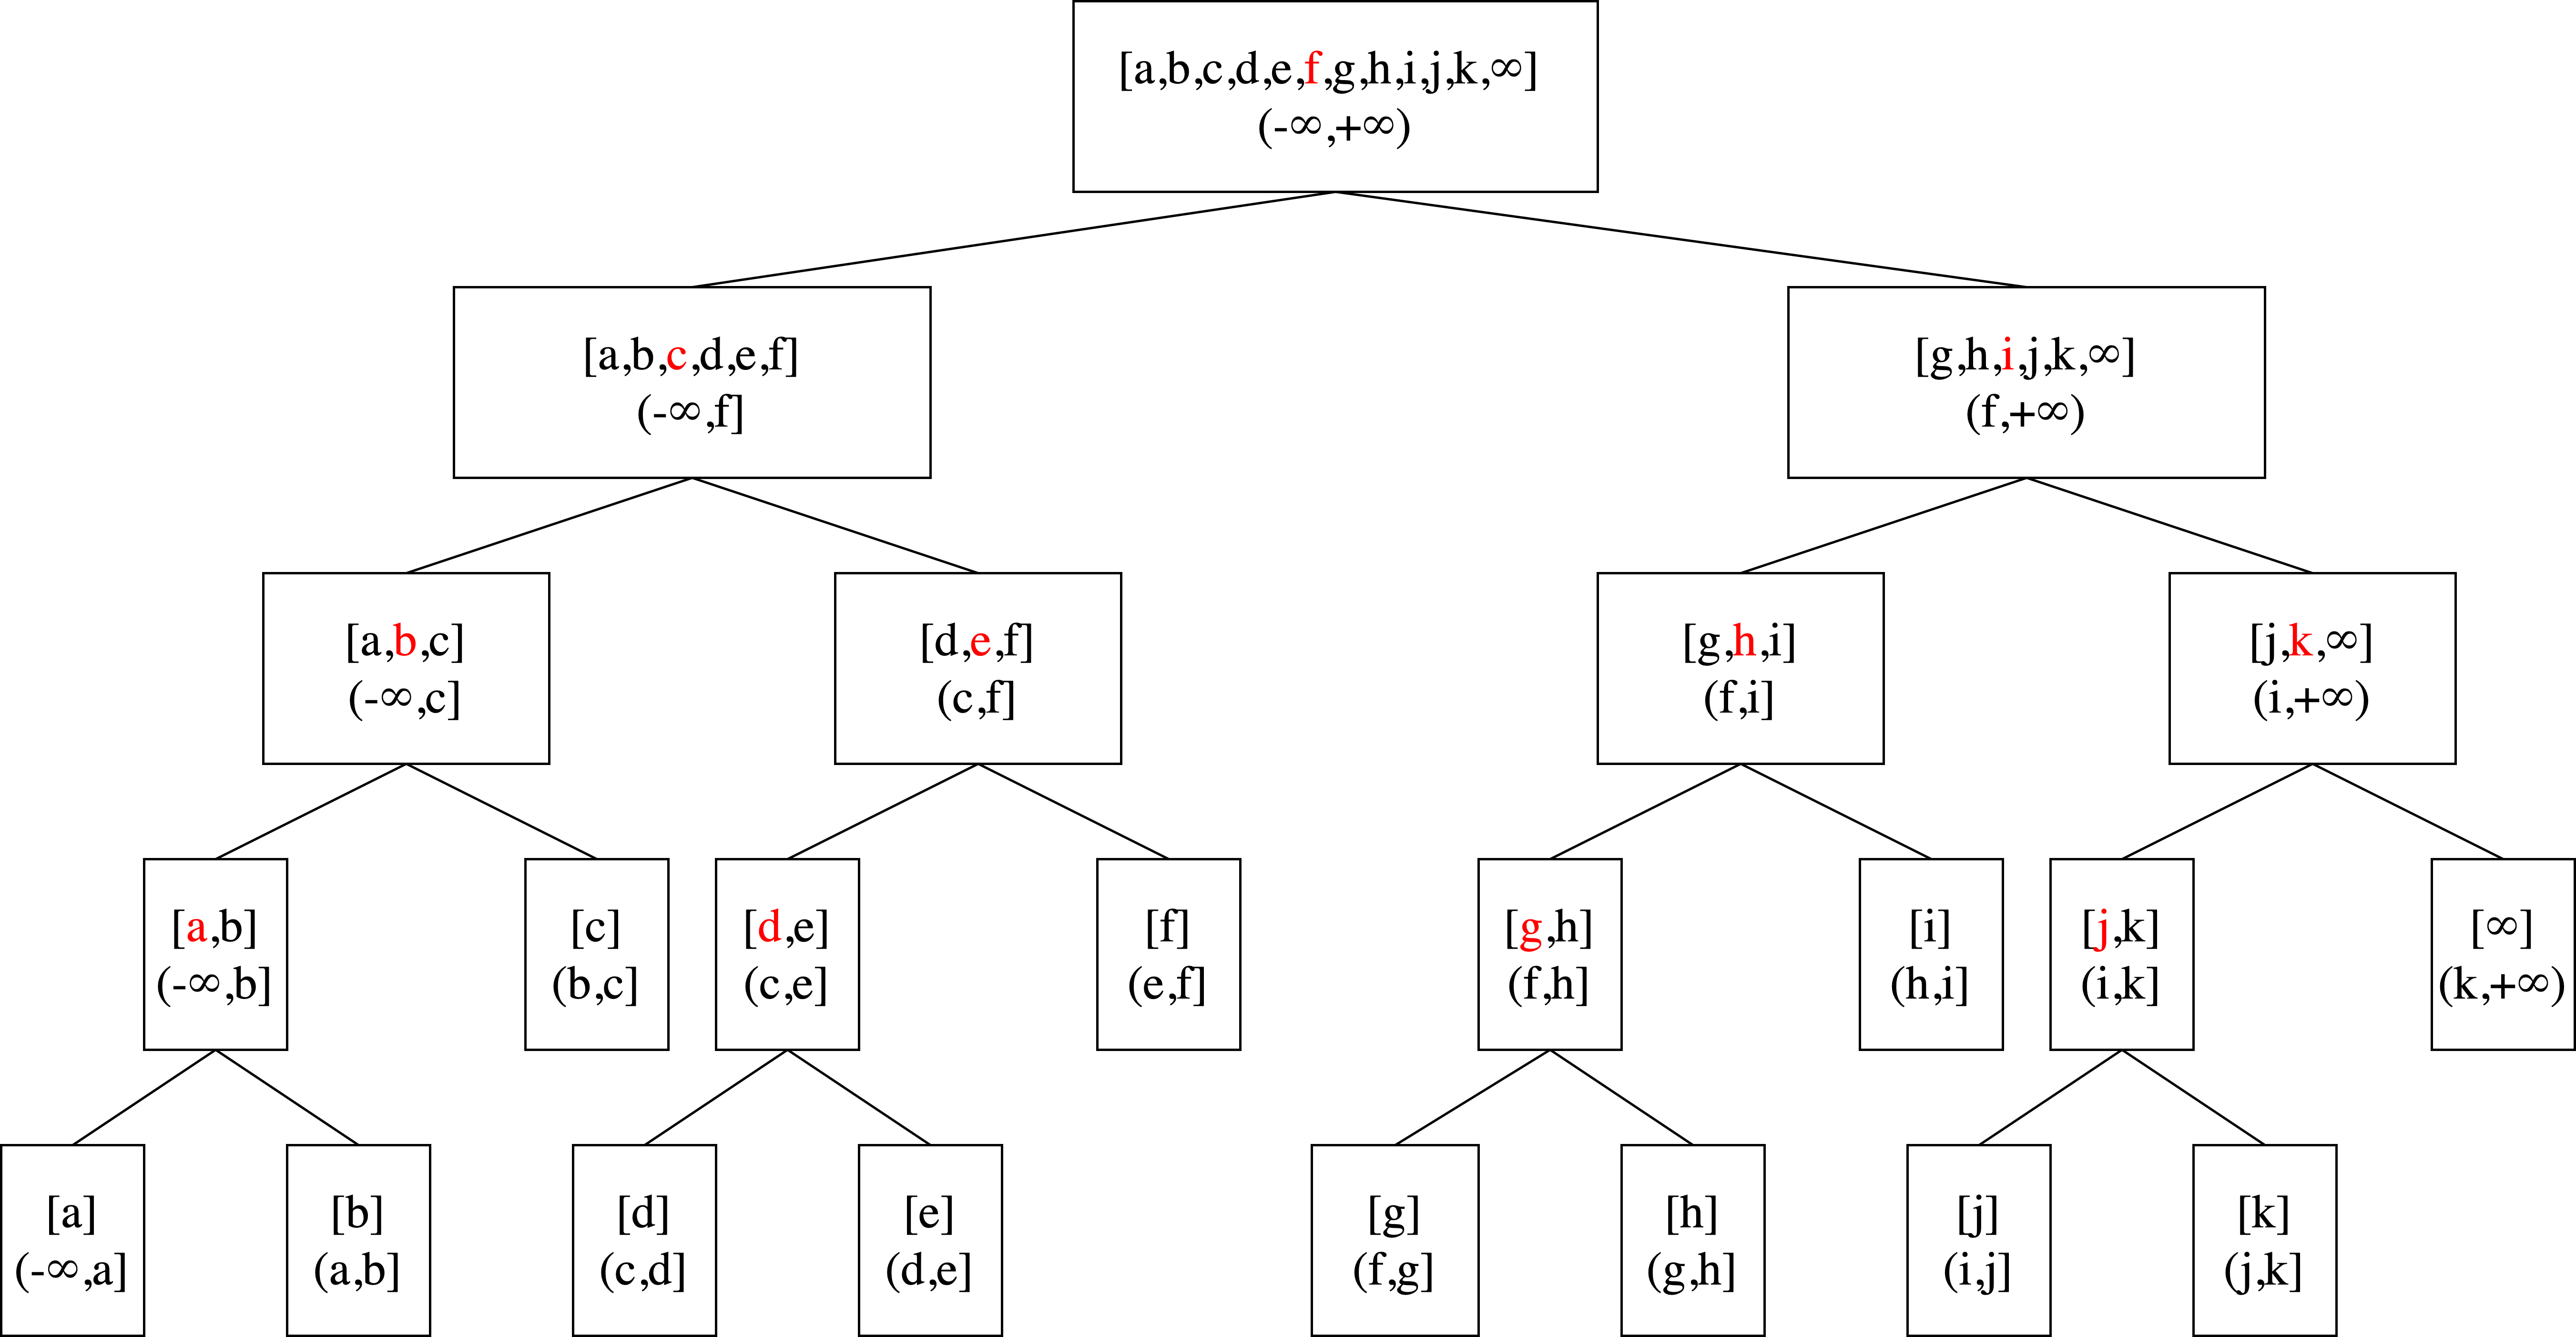
\includegraphics[scale=0.05]{ClusterGraph}
\end{center}

The point where a node divides the array into two parts is at the midpoint of the array (the red value) and can be null if the node is a leaf. K such values (one per dimension) form a DataPoint object and this DataPoint object is called the anchor of this node.

\subsubsection{Building The Tree}

DFS is used here to populate all the children of a node. When populating the children for a node, it first populates the two children in dimension 0, then the two children in dimension 1, …

When a node is trying to add a child, either left or right, to a node, it first computes the range of the child node, then uses \(ClusterGraph.search()\) to check whether this node has been added to the graph. If so, we only “link” the two nodes. Otherwise, we initiate a child Cluster object and “link” them.

\subsubsection{Processing Data Points}

We will feed the data in, A DataPoint object is created for each row of data. Each DataPoint object travels from the root Cluster to a Cluster that is a leaf in every dimension and increase the count value of every node in the middle by 1. Because the traversal can has multiple paths, We avoid duplicate visiting by using a flag of the Cluster object.

\subsection{DataParser}
The DataParser class is constructed from a Config object.  From the Config, The DataParser extracts the configuration parameters specific to the input dataset including:
\begin{itemize}
    \item The line of the input dataset file to begin reading from.
    \item The columns of the input dataset to use for the clustering.
    \item The path to the input dataset file.
    \item Number of data points to read into the cluster graph at a time, i.e. batch size.
    \item How to handle missing/null values for rows in the data set.
\end{itemize}
The user must specify all of these parameters in the configuration file before trying to process the dataset.  When all the required parameters are supplied, the DataParser is ready to read the input file and feed batches to the cluster graph.

\subsection{Reporter}
The Reporter class is responsible for compressing the ClusterGraph, identifying the noteworthy clustering, and outputting them into a human-readable text file. The Reporter class is constructed using a Config object and a ClusterGraph. From the Config, the Reporter extracts the predefined threshold and the path to the file that will contain the report.

To compress the graph, our algorithm eliminates unimportant clusters by traversing the tree and pruning any subtrees whose root is less than the threshold. After that, the compress report algorithm given below is applied to the pruned graph to identify the noteworthy clusters through a bottom-up traversal, where a cluster is included only if it contains a significant amount of data not contained in its already reported descendants. This is determined by an estimate calculation also employing the threshold. Finally, the list of significant clusters is formatted and written to an output file.


\begin{center}
   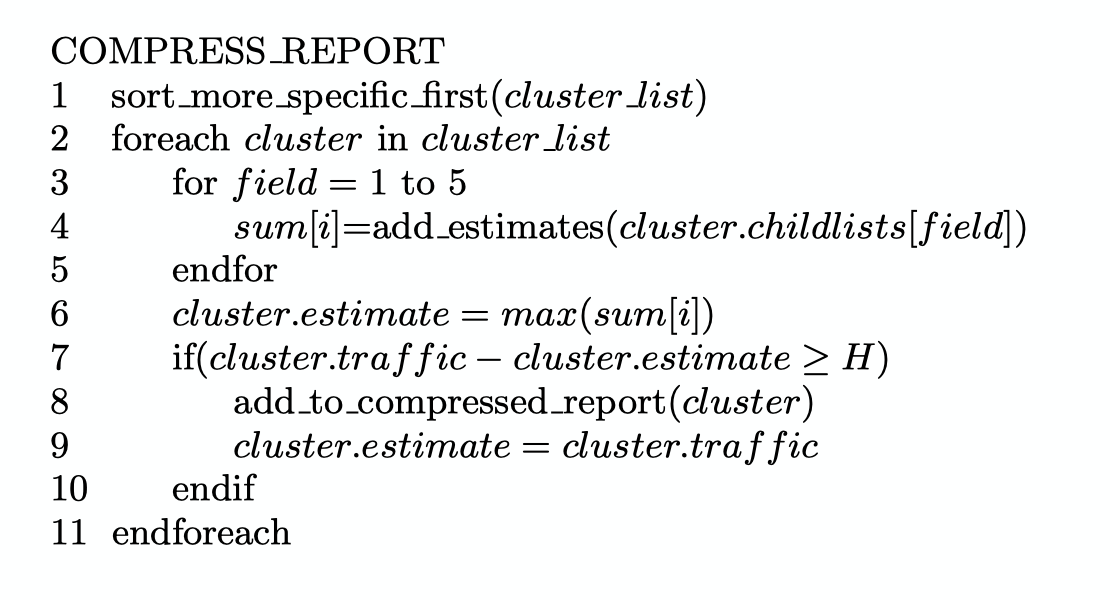
\includegraphics[scale=0.5]{CompressGraph}
\end{center}

\section{Experiment}
The dataset we chose to evaluate the implementation was created by Google to track mobility flows during the COVID-19 Pandemic. A link to download this data is in the GitHub repository for this project.  The dataset is formatted as the following (Note: R/R is Retail and Recreation and G/P is Grocery and Pharmacy),

\begin{adjustbox}{width=\textwidth,totalheight=\textheight,keepaspectratio,rotate=0,caption={Data Format},nofloat=table}
\begin{tabular}{ |c|c|c|c|c|c|c|c|c| }
\hline
 Country & ... &Date&R/R&G/P&Parks&Transit&Workplaces&Residential \\ 
 \hline
 AE&...&2020-02-15&0&4&5&0&2&1 \\
 US&...&2020-06-07&-12&0&54&-8&-6&4 \\
 VN&...&2020-03-23&-34&-18&-32&-42&-1&9 \\
 ...&...&...&...&...&...&...&...&... \\
 \hline
\end{tabular}
\end{adjustbox}

\hfill

For columns R/R through Residential the value represents a percentage change from that particular location's baseline.  The value could be in the range \([-100, \infty)\).

Due to our implementation currently only supporting ranges, when processing the data we ignore all purely categorical columns including Country and number of omitted miscellaneous columns between Country and Date.  For our experimentation we will only focus on columns Date through Residential.  We are are aware that this choice to abstract region from the algorithm will cause a loss of potentially meaningful results regarding the locality of the high volume clusters, however for the sake of computational complexity viewing this abstraction as a measurement of the global mobility flows is sufficient.  As of June 6th, 2020 the dataset contains approximately 517,000 data points.

\hfill

The main program will execute the simple flow illustrated below.
\begin{center}
\tikzstyle{startstop} = [rectangle, rounded corners, minimum width=3cm, minimum height=0.6cm,text centered, draw=black]
\tikzstyle{arrow} = [thick,->,>=stealth]
    \begin{tikzpicture}[node distance=1cm]
\node (start) [startstop] {Load user specified Config from file};
\node (in1) [startstop, below of=start] {Create and Populate ClusterGraph based on Config};
\node (in2) [startstop, below of=in1] {Create DataParser with Config and feed data batches to ClusterGraph};
\node (in3) [startstop, below of=in2] {Create Reporter with Config and ClusterGraph};
\node (in4) [startstop, below of=in3] {With Reporter, perform compression and generate the report};
\draw [arrow] (start) -- (in1);
\draw [arrow] (in1) -- (in2);
\draw [arrow] (in2) -- (in3);
\draw [arrow] (in3) -- (in4);
\end{tikzpicture}
\end{center}

\hfill

We will run the algorithm on the input dataset with varying parameters in the configuration file to see if we can draw any interesting conclusions from the global mobility dataset.

\section{Results}
To demonstrate the flexibility of the algorithm, we will produce results on three different configurations:
\begin{itemize}
    \item Greater than two date ranges and only positive or negative flows.
    \item Two date ranges and multiple ranges for flows.
    \item Greater than two date ranges and and multiple ranges for flows.
\end{itemize}

For each configuration, we will produce results setting the threshold to 10,000.  If any null fields in a data point are encountered, the data point will be omitted.

\subsection{Demo Configuration 1}
\begin{center}
\footnotesize{
\begin{lstlisting}
DATA_INDICES=6,7,8,9,10,11,12
DATA_TYPES=DATA_DATE,DATA_INT,DATA_INT,DATA_INT,DATA_INT,DATA_INT,DATA_INT
CUTOFF_VALS=[2020-03-05,2020-04-07,2020-05-11],[0],[0],[0],[0],[0],[0]
\end{lstlisting}
}
\end{center}

This threshold value reported \textbf{91} clusters meeting this configuration.  To keep this table brief only the top 10 clusters will be shown in this table.  The full report can be seen under the examples section in the GitHub repository.
\newline
\begin{adjustbox}{width=\textwidth,totalheight=\textheight,keepaspectratio,rotate=0,caption={Demo Configuration 1 - Results},nofloat=table}
\begin{tabular}{ |p{0.08\linewidth}|p{0.38\linewidth}|p{0.1\linewidth}|p{0.1\linewidth}|p{0.1\linewidth}|p{0.1\linewidth}|p{0.15\linewidth}|p{0.15\linewidth}| }
\hline
Count&Date&R/R&G/P&Parks&Transit&Workplaces&Residential \\
\hline
101533&\((-\infty,\infty)\)&\((-\infty,\infty)\)&\((-\infty,\infty)\)&\((-\infty,0]\)&\((-\infty,\infty)\)&\((-\infty,\infty)\)&\((0,\infty)\) \\
\hline
89949&\((-\infty,\infty)\)&\((-\infty,0]\)&\((-\infty,\infty)\)&\((-\infty,0]\)&\((-\infty,0]\)&\((-\infty,0]\)&\((0,\infty)\) \\
\hline
89832&\((-\infty,\infty)\)&\((-\infty,0]\)&\((-\infty,0]\)&\((-\infty,0]\)&\((-\infty,\infty)\)&\((-\infty,\infty)\)&\((-\infty,\infty)\) \\
\hline
47725&\((2020-03-05,2020-04-07]\)&\((-\infty,\infty)\)&\((-\infty,\infty)\)&\((-\infty,\infty)\)&\((-\infty,0]\)&\((-\infty,\infty)\)&\((-\infty,\infty)\) \\
\hline
47635&\((2020-03-05,2020-04-07]\)&\((-\infty,\infty)\)&\((-\infty,\infty)\)&\((-\infty,\infty)\)&\((-\infty,\infty)\)&\((-\infty,\infty)\)&\((0,\infty)\) \\
\hline
39318&\((2020-05-11,\infty)\)&\((-\infty,0]\)&\((-\infty,\infty)\)&\((-\infty,\infty)\)&\((-\infty,0]\)&\((-\infty,\infty)\)&\((-\infty,\infty)\) \\
\hline
39315&\((2020-05-11,\infty)\)&\((-\infty,\infty)\)&\((-\infty,\infty)\)&\((-\infty,\infty)\)&\((-\infty,0]\)&\((-\infty,\infty)\)&\((0,\infty)\) \\
\hline
38853&\((2020-05-11,\infty)\)&\((-\infty,0]\)&\((-\infty,\infty)\)&\((-\infty,\infty)\)&\((-\infty,\infty)\)&\((-\infty,0]\)&\((-\infty,\infty)\) \\
\hline
38665&\((-\infty,2020-04-07]\)&\((-\infty,0]\)&\((-\infty,0]\)&\((-\infty,\infty)\)&\((-\infty,0]\)&\((-\infty,\infty)\)&\((0,\infty)\) \\
\hline
\end{tabular}
\end{adjustbox}


\subsection{Demo Configuration 2}
\begin{center}
\footnotesize{
\begin{lstlisting}
DATA_INDICES=6,7,8,9,10,11,12
DATA_TYPES=DATA_DATE,DATA_INT,DATA_INT,DATA_INT,DATA_INT,DATA_INT,DATA_INT
CUTOFF_VALS=[2020-04-07],[0],[0],[0],[0],[0],[-10,0,10]
\end{lstlisting}
}
\end{center}

This threshold value reported \textbf{83} clusters meeting this configuration.  To keep this table brief only the top 10 clusters will be shown in this table.

\hfill
\begin{adjustbox}{width=\textwidth,totalheight=\textheight,keepaspectratio,rotate=0,caption={Demo Configuration 2 - Results},nofloat=table}
\begin{tabular}{ |p{0.08\linewidth}|p{0.38\linewidth}|p{0.1\linewidth}|p{0.1\linewidth}|p{0.1\linewidth}|p{0.1\linewidth}|p{0.15\linewidth}|p{0.15\linewidth}| }
\hline
Count&Date&R/R&G/P&Parks&Transit&Workplaces&Residential \\
\hline
123556&\((-\infty,\infty)\)&\((-\infty,0]\)&\((-\infty,0]\)&\((-\infty,\infty)\)&\((-\infty,\infty)\)&\((-\infty,\infty)\)&\((-\infty,\infty)\) \\
\hline
91768&\((-\infty,\infty)\)&\((-\infty,\infty)\)&\((-\infty,0]\)&\((-\infty,0]\)&\((-\infty,\infty)\)&\((-\infty,\infty)\)&\((-\infty,\infty)\) \\
\hline
91450&\((-\infty,\infty)\)&\((-\infty,\infty)\)&\((-\infty,\infty)\)&\((-\infty,0]\)&\((-\infty,0]\)&\((-\infty,0]\)&\((-\infty,\infty)\) \\
\hline
91370&\((-\infty,\infty)\)&\((-\infty,0]\)&\((-\infty,\infty)\)&\((-\infty,0]\)&\((-\infty,\infty)\)&\((-\infty,0]\)&\((0,\infty)\) \\
\hline
60447&\((-\infty,2020-04-07]\)&\((-\infty,\infty)\)&\((-\infty,\infty)\)&\((-\infty,\infty)\)&\((-\infty,\infty)\)&\((-\infty,\infty)\)&\((0,\infty)\) \\
\hline
59887&\((2020-04-07,\infty)\)&\((-\infty,0]\)&\((-\infty,\infty)\)&\((-\infty,0]\)&\((-\infty,0]\)&\((-\infty,\infty)\)&\((0,\infty)\) \\
\hline
58618&\((2020-04-07,\infty)\)&\((-\infty,\infty)\)&\((-\infty,\infty)\)&\((-\infty,0]\)&\((-\infty,\infty)\)&\((-\infty,0]\)&\((-\infty,\infty)\) \\
\hline
48550&\((2020-04-07,\infty)\)&\((-\infty,0]\)&\((-\infty,0]\)&\((-\infty,0]\)&\((-\infty,0]\)&\((-\infty,0]\)&\((10,\infty)\) \\
\hline
36374&\((-\infty,\infty)\)&\((-\infty,\infty)\)&\((-\infty,\infty)\)&\((-\infty,\infty)\)&\((-\infty,0]\)&\((-\infty,0]\)&\((0,10]\) \\
\hline
36082&\((-\infty,\infty)\)&\((-\infty,0]\)&\((-\infty,\infty)\)&\((-\infty,\infty)\)&\((-\infty,\infty)\)&\((-\infty,0]\)&\((0,10]\) \\
\hline
\end{tabular}
\end{adjustbox}

\subsection{Demo Configuration 3}
\begin{center}
\footnotesize{
\begin{lstlisting}
DATA_INDICES=6,7,8,9,10,11,12
DATA_TYPES=DATA_DATE,DATA_INT,DATA_INT,DATA_INT,DATA_INT,DATA_INT,DATA_INT
CUTOFF_VALS=[2020-03-05,2020-04-07,2020-05-11],[0],[0],[0],[0],[0],[-10,0,10]
\end{lstlisting}
}
\end{center}
This threshold value reported \textbf{119} clusters meeting this configuration.  To keep this table brief only the top 10 clusters will be shown in this table.

\hfill
\begin{adjustbox}{width=\textwidth,totalheight=\textheight,keepaspectratio,rotate=0,caption={Demo Configuration 3 - Results},nofloat=table}
\begin{tabular}{ |p{0.08\linewidth}|p{0.38\linewidth}|p{0.1\linewidth}|p{0.1\linewidth}|p{0.1\linewidth}|p{0.1\linewidth}|p{0.15\linewidth}|p{0.15\linewidth}| }
\hline
Count&Date&R/R&G/P&Parks&Transit&Workplaces&Residential \\
\hline
121100&\((-\infty,\infty)\)&\((-\infty,\infty)\)&\((-\infty,0]\)&\((-\infty,\infty)\)&\((-\infty,\infty)\)&\((-\infty,\infty)\)&\((0,\infty)\) \\
\hline
119653&\((-\infty,\infty)\)&\((-\infty,0]\)&\((-\infty,0]\)&\((-\infty,\infty)\)&\((-\infty,0]\)&\((-\infty,\infty)\)&\((-\infty,\infty)\) \\
\hline
91768&\((-\infty,\infty)\)&\((-\infty,\infty)\)&\((-\infty,0]\)&\((-\infty,0]\)&\((-\infty,\infty)\)&\((-\infty,\infty)\)&\((-\infty,\infty)\) \\
\hline
91450&\((-\infty,\infty)\)&\((-\infty,\infty)\)&\((-\infty,\infty)\)&\((-\infty,0]\)&\((-\infty,0]\)&\((-\infty,0]\)&\((-\infty,\infty)\) \\
\hline
91370&\((-\infty,\infty)\)&\((-\infty,0]\)&\((-\infty,\infty)\)&\((-\infty,0]\)&\((-\infty,\infty)\)&\((-\infty,0]\)&\((0,\infty)\) \\
\hline
59887&\((2020-04-07,\infty)\)&\((-\infty,0]\)&\((-\infty,\infty)\)&\((-\infty,0]\)&\((-\infty,0]\)&\((-\infty,\infty)\)&\((0,\infty)\) \\
\hline
58618&\((2020-04-07,\infty)\)&\((-\infty,\infty)\)&\((-\infty,\infty)\)&\((-\infty,0]\)&\((-\infty,\infty)\)&\((-\infty,0]\)&\((-\infty,\infty)\) \\
\hline
55267&\((2020-03-05,2020-04-07]\)&\((-\infty,\infty)\)&\((-\infty,\infty)\)&\((-\infty,\infty)\)&\((-\infty,\infty)\)&\((-\infty,\infty)\)&\((-\infty,\infty)\) \\
\hline
44087&\((-\infty,2020-04-07]\)&\((-\infty,0]\)&\((-\infty,0]\)&\((-\infty,\infty)\)&\((-\infty,\infty)\)&\((-\infty,\infty)\)&\((-\infty,\infty)\) \\
\hline
43525&\((2020-04-07,2020-05-11]\)&\((-\infty,0]\)&\((-\infty,0]\)&\((-\infty,\infty)\)&\((-\infty,0]\)&\((-\infty,\infty)\)&\((10,\infty)\) \\
\hline
\end{tabular}
\end{adjustbox}

\subsection{Results Analysis}
The intuition to draw from each of these results can be done by first looking at the highest volume cluster.  In Configuration 1 the highest volume cluster has a count of 101533.  A significant portion of the dataset passed through this node and it is safe to say, while not being overly specific, this is a dominant trend in the dataset.  This cluster does not have any significant volume in the date ranges we specified in the configurations so this cluster represents the entire date range of the dataset.  The \((-\infty, \infty)\) is synonymous to the root cluster in that dimension.  The most interesting results are the columns that do not specify the root cluster. For the highest volume cluster in Configuration 1 the non-root clusters are Parks and Residential which are \((-\infty, 0]\) and \((0, \infty)\) respectively.  These ranges indicate the most dominant trend was there was a decrease in travel to Parks and an increase in travel in Residential areas.  This is consistent with the stay-home-orders issued during the peak of the pandemic.  The lower volume clusters on the top ten begin to describe clusters with more specific features.  For example, in Configuration 3 the tenth highest cluster with a volume of 43525 shows that between April 7th and May 5th there was a global decrease in Restaurants and Retail, Grocery and Pharmacy , and Transit Stations.  However, this cluster specifically shows the increase in Residential mobility was at least greater than 10 percent.  This result provides more insight into the data given the specificity of the date and residential ranges.
\newline
\newline
The are many configurations one could use to cluster this dataset.  A person with a great deal of domain knowledge for a given dataset could supply an interesting configuration to produce results allowing them to draw conclusions they would not have otherwise been able to inspecting the dataset manually.  

\section{Conclusion}
We believe we have created an easy to use, extensible implementation of this scalable clustering algorithm that can be applied to many datasets. We believe this tool can be useful to large datasets, but from our experience there are several limitations. One limitation of this approach is that users must predefine the cutoff values used for clustering the data and the threshold used to identify noteworthy clusters. This requires a lot of domain knowledge and time to manually tune the parameters to find interesting results. Another limitation is that it is difficult to create a useful visualization of the results that can apply to any dataset with a variable number of features. This led us to display the results in a simple tabular form, but this can be difficult to interpret without domain specific knowledge. Nonetheless, this algorithm can be a powerful tool for processing large amounts of data and we hope that our implementation can be used by developers going forward.

\bibliography{references}

\end{document}
